\documentclass{standalone}
\usepackage{tikz}
\usetikzlibrary{patterns, positioning}

\begin{document}
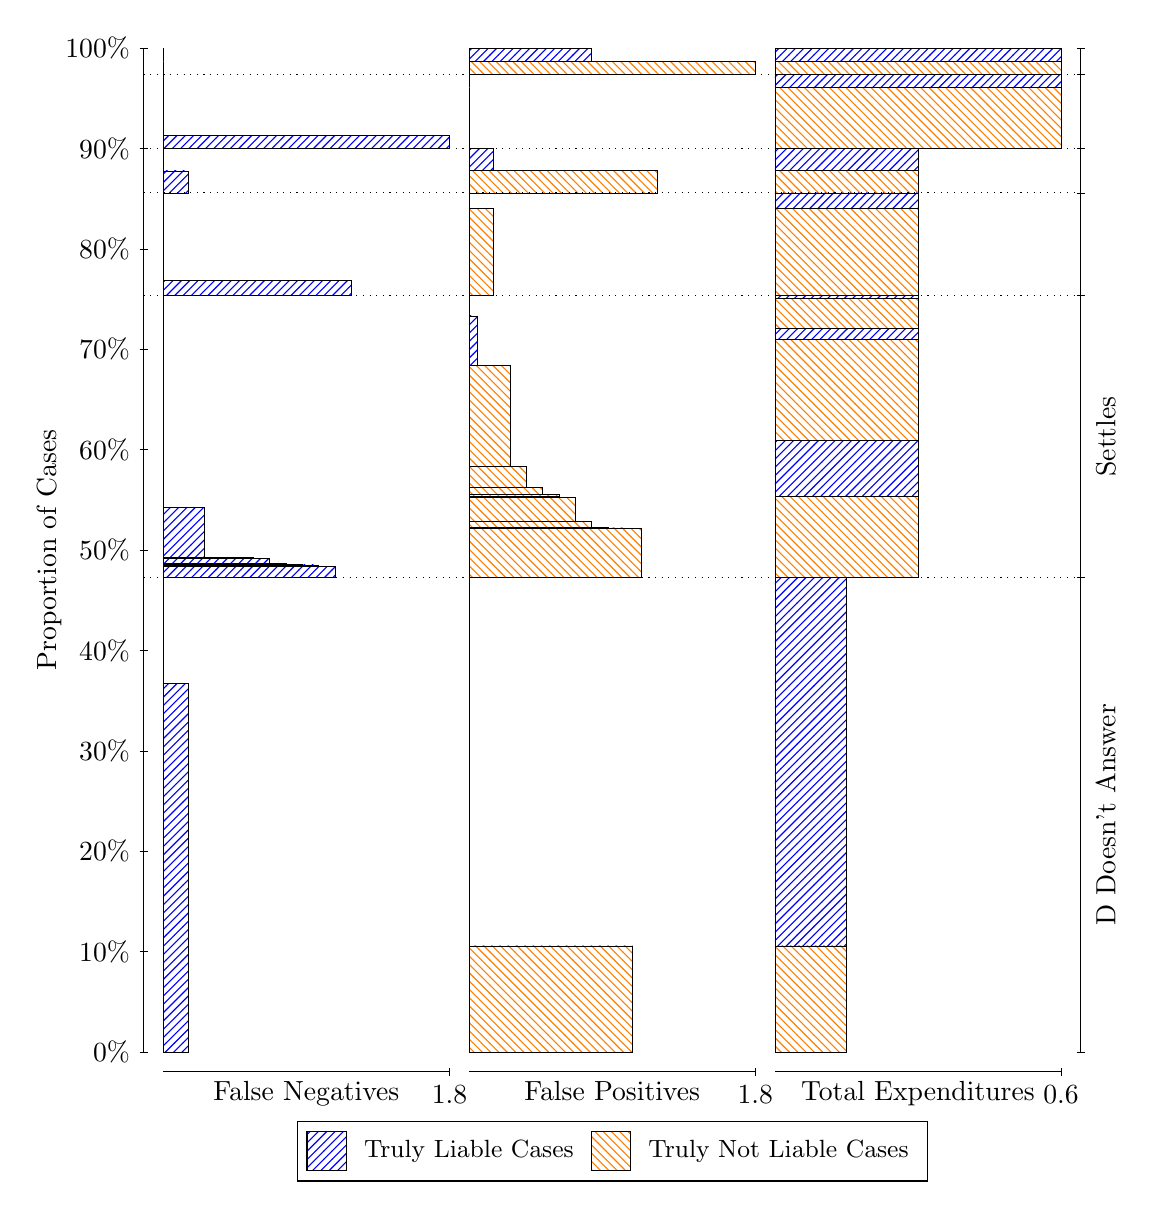
\begin{tikzpicture}
\draw[black, very thin] (1.5,1.75) -- (1.5,14.5);
\node[rotate=90, anchor=center] at (0.3, 8.125) {Proportion of Cases};
\draw[black, very thin] (1.45,1.75) -- (1.55,1.75);
\node[anchor=east] at (1.45, 1.75) {0\%};
\draw[black, very thin] (1.45,3.025) -- (1.55,3.025);
\node[anchor=east] at (1.45, 3.025) {10\%};
\draw[black, very thin] (1.45,4.3) -- (1.55,4.3);
\node[anchor=east] at (1.45, 4.3) {20\%};
\draw[black, very thin] (1.45,5.575) -- (1.55,5.575);
\node[anchor=east] at (1.45, 5.575) {30\%};
\draw[black, very thin] (1.45,6.85) -- (1.55,6.85);
\node[anchor=east] at (1.45, 6.85) {40\%};
\draw[black, very thin] (1.45,8.125) -- (1.55,8.125);
\node[anchor=east] at (1.45, 8.125) {50\%};
\draw[black, very thin] (1.45,9.4) -- (1.55,9.4);
\node[anchor=east] at (1.45, 9.4) {60\%};
\draw[black, very thin] (1.45,10.675) -- (1.55,10.675);
\node[anchor=east] at (1.45, 10.675) {70\%};
\draw[black, very thin] (1.45,11.95) -- (1.55,11.95);
\node[anchor=east] at (1.45, 11.95) {80\%};
\draw[black, very thin] (1.45,13.225) -- (1.55,13.225);
\node[anchor=east] at (1.45, 13.225) {90\%};
\draw[black, very thin] (1.45,14.5) -- (1.55,14.5);
\node[anchor=east] at (1.45, 14.5) {100\%};

\draw[black, very thin] (13.4,1.75) -- (13.4,14.5);
\draw[black, very thin] (13.35,1.75) -- (13.45,1.75);
\node[anchor=west] at (13.35, 1.75) {};
\draw[black, very thin] (13.35,7.7734) -- (13.45,7.7734);
\node[anchor=west] at (13.35, 7.7734) {};
\draw[black, very thin] (13.35,11.358) -- (13.45,11.358);
\node[anchor=west] at (13.35, 11.358) {};
\draw[black, very thin] (13.35,12.661) -- (13.45,12.661);
\node[anchor=west] at (13.35, 12.661) {};
\draw[black, very thin] (13.35,13.227) -- (13.45,13.227);
\node[anchor=west] at (13.35, 13.227) {};
\draw[black, very thin] (13.35,14.167) -- (13.45,14.167);
\node[anchor=west] at (13.35, 14.167) {};
\draw[black, very thin] (13.35,14.5) -- (13.45,14.5);
\node[anchor=west] at (13.35, 14.5) {};

\draw[black, very thin, pattern color=blue, pattern=north east lines] (1.75,1.75) rectangle (2.0614,6.4273);
\draw[black, very thin, pattern color=orange, pattern=north west lines] (1.75,6.4273) rectangle (1.75,7.7734);
\draw[black, very thin, pattern color=blue, pattern=north east lines] (1.75,7.7734) rectangle (3.93,7.9126);
\draw[black, very thin, pattern color=blue, pattern=north east lines] (1.75,7.9126) rectangle (3.7224,7.9369);
\draw[black, very thin, pattern color=blue, pattern=north east lines] (1.75,7.9369) rectangle (3.5148,7.9459);
\draw[black, very thin, pattern color=blue, pattern=north east lines] (1.75,7.9459) rectangle (3.3071,7.9501);
\draw[black, very thin, pattern color=blue, pattern=north east lines] (1.75,7.9501) rectangle (3.0995,8.0153);
\draw[black, very thin, pattern color=blue, pattern=north east lines] (1.75,8.0153) rectangle (2.8919,8.0297);
\draw[black, very thin, pattern color=blue, pattern=north east lines] (1.75,8.0297) rectangle (2.6843,8.0322);
\draw[black, very thin, pattern color=blue, pattern=north east lines] (1.75,8.0322) rectangle (2.4767,8.0347);
\draw[black, very thin, pattern color=blue, pattern=north east lines] (1.75,8.0347) rectangle (2.269,8.6625);
\draw[black, very thin, pattern color=orange, pattern=north west lines] (1.75,8.6625) rectangle (1.75,11.358);
\draw[black, very thin, pattern color=blue, pattern=north east lines] (1.75,11.358) rectangle (4.1376,11.553);
\draw[black, very thin, pattern color=orange, pattern=north west lines] (1.75,11.553) rectangle (1.75,12.661);
\draw[black, very thin, pattern color=blue, pattern=north east lines] (1.75,12.661) rectangle (2.0614,12.939);
\draw[black, very thin, pattern color=orange, pattern=north west lines] (1.75,12.939) rectangle (1.75,13.227);
\draw[black, very thin, pattern color=blue, pattern=north east lines] (1.75,13.227) rectangle (5.3833,13.393);
\draw[black, very thin, pattern color=orange, pattern=north west lines] (1.75,13.393) rectangle (1.75,14.167);
\draw[black, very thin, pattern color=orange, pattern=north west lines] (1.75,14.167) rectangle (1.75,14.329);
\draw[black, very thin, pattern color=blue, pattern=north east lines] (1.75,14.329) rectangle (1.75,14.5);
\draw[black, very thin, pattern color=orange, pattern=north west lines] (5.6333,1.75) rectangle (7.7095,3.096);
\draw[black, very thin, pattern color=blue, pattern=north east lines] (5.6333,3.096) rectangle (5.6333,7.7734);
\draw[black, very thin, pattern color=orange, pattern=north west lines] (5.6333,7.7734) rectangle (7.8133,8.4003);
\draw[black, very thin, pattern color=orange, pattern=north west lines] (5.6333,8.4003) rectangle (7.6057,8.4062);
\draw[black, very thin, pattern color=orange, pattern=north west lines] (5.6333,8.4062) rectangle (7.3981,8.4125);
\draw[black, very thin, pattern color=orange, pattern=north west lines] (5.6333,8.4125) rectangle (7.1905,8.4854);
\draw[black, very thin, pattern color=orange, pattern=north west lines] (5.6333,8.4854) rectangle (6.9829,8.7981);
\draw[black, very thin, pattern color=orange, pattern=north west lines] (5.6333,8.7981) rectangle (6.7752,8.8036);
\draw[black, very thin, pattern color=orange, pattern=north west lines] (5.6333,8.8036) rectangle (6.7752,8.8277);
\draw[black, very thin, pattern color=orange, pattern=north west lines] (5.6333,8.8277) rectangle (6.5676,8.9167);
\draw[black, very thin, pattern color=orange, pattern=north west lines] (5.6333,8.9167) rectangle (6.36,9.1858);
\draw[black, very thin, pattern color=orange, pattern=north west lines] (5.6333,9.1858) rectangle (6.1524,10.469);
\draw[black, very thin, pattern color=blue, pattern=north east lines] (5.6333,10.469) rectangle (5.7371,11.097);
\draw[black, very thin, pattern color=blue, pattern=north east lines] (5.6333,11.097) rectangle (5.6333,11.358);
\draw[black, very thin, pattern color=orange, pattern=north west lines] (5.6333,11.358) rectangle (5.9448,12.466);
\draw[black, very thin, pattern color=blue, pattern=north east lines] (5.6333,12.466) rectangle (5.6333,12.661);
\draw[black, very thin, pattern color=orange, pattern=north west lines] (5.6333,12.661) rectangle (8.021,12.95);
\draw[black, very thin, pattern color=blue, pattern=north east lines] (5.6333,12.95) rectangle (5.9448,13.227);
\draw[black, very thin, pattern color=orange, pattern=north west lines] (5.6333,13.227) rectangle (5.6333,14.001);
\draw[black, very thin, pattern color=blue, pattern=north east lines] (5.6333,14.001) rectangle (5.6333,14.167);
\draw[black, very thin, pattern color=orange, pattern=north west lines] (5.6333,14.167) rectangle (9.2667,14.329);
\draw[black, very thin, pattern color=blue, pattern=north east lines] (5.6333,14.329) rectangle (7.1905,14.5);
\draw[black, very thin, pattern color=orange, pattern=north west lines] (9.5167,1.75) rectangle (10.425,3.096);
\draw[black, very thin, pattern color=blue, pattern=north east lines] (9.5167,3.096) rectangle (10.425,7.7734);
\draw[black, very thin, pattern color=orange, pattern=north west lines] (9.5167,7.7734) rectangle (11.333,8.8036);
\draw[black, very thin, pattern color=blue, pattern=north east lines] (9.5167,8.8036) rectangle (11.333,9.5168);
\draw[black, very thin, pattern color=orange, pattern=north west lines] (9.5167,9.5168) rectangle (11.333,10.8);
\draw[black, very thin, pattern color=blue, pattern=north east lines] (9.5167,10.8) rectangle (11.333,10.939);
\draw[black, very thin, pattern color=orange, pattern=north west lines] (9.5167,10.939) rectangle (11.333,11.321);
\draw[black, very thin, pattern color=blue, pattern=north east lines] (9.5167,11.321) rectangle (11.333,11.358);
\draw[black, very thin, pattern color=orange, pattern=north west lines] (9.5167,11.358) rectangle (11.333,12.466);
\draw[black, very thin, pattern color=blue, pattern=north east lines] (9.5167,12.466) rectangle (11.333,12.661);
\draw[black, very thin, pattern color=orange, pattern=north west lines] (9.5167,12.661) rectangle (11.333,12.95);
\draw[black, very thin, pattern color=blue, pattern=north east lines] (9.5167,12.95) rectangle (11.333,13.227);
\draw[black, very thin, pattern color=orange, pattern=north west lines] (9.5167,13.227) rectangle (13.15,14.001);
\draw[black, very thin, pattern color=blue, pattern=north east lines] (9.5167,14.001) rectangle (13.15,14.167);
\draw[black, very thin, pattern color=orange, pattern=north west lines] (9.5167,14.167) rectangle (13.15,14.329);
\draw[black, very thin, pattern color=blue, pattern=north east lines] (9.5167,14.329) rectangle (13.15,14.5);
\draw[black, dotted] (1.5,7.7734) -- (13.4,7.7734);
\draw[black, dotted] (1.5,11.358) -- (13.4,11.358);
\draw[black, dotted] (1.5,12.661) -- (13.4,12.661);
\draw[black, dotted] (1.5,13.227) -- (13.4,13.227);
\draw[black, dotted] (1.5,14.167) -- (13.4,14.167);
\draw[black, very thin] (1.75,1.5) -- (5.3833,1.5);
\node[anchor=north] at (3.5667, 1.5) {False Negatives};
\draw[black, very thin] (5.3833,1.45) -- (5.3833,1.55);
\node[anchor=north] at (5.3833, 1.45) {1.8};

\draw[black, very thin] (5.6333,1.5) -- (9.2667,1.5);
\node[anchor=north] at (7.45, 1.5) {False Positives};
\draw[black, very thin] (9.2667,1.45) -- (9.2667,1.55);
\node[anchor=north] at (9.2667, 1.45) {1.8};

\draw[black, very thin] (9.5167,1.5) -- (13.15,1.5);
\node[anchor=north] at (11.333, 1.5) {Total Expenditures};
\draw[black, very thin] (13.15,1.45) -- (13.15,1.55);
\node[anchor=north] at (13.15, 1.45) {0.6};

\node[black, centered, rotate=90] at (13.72, 4.7617) {D Doesn't Answer};
\node[black, centered, rotate=90] at (13.72, 9.5658) {Settles};





\draw (7.449999999999999,1.5) node[draw=none] (baseCoordinate) {};
\begin{scope}[align=center]
        \matrix[scale=0.5, draw=black, below=0.5cm of baseCoordinate, nodes={draw}, column sep=0.1cm]{
            \node[rectangle, draw, minimum width=0.5cm, minimum height=0.5cm, pattern=north east lines, pattern color=blue] {}; &
            \node[draw=none, font=\small] (B) {Truly Liable Cases}; &
            \node[rectangle, draw, minimum width=0.5cm, minimum height=0.5cm, pattern=north west lines, pattern color=orange] {}; &
            \node[draw=none, font=\small] (B) {Truly Not Liable Cases}; \\
            };
\end{scope}

\end{tikzpicture}
\end{document}